

% \input{Preliminaries}
% \subsection{RMPA neuron}
% The core spiking logic of this paradigm is the amplification mechanism of the residual membrane potential. We believe that instead of accumulating through a large number of cycles to reduce the residual membrane potential per cycle, it is better to directly amplify the residual membrane potential so that the proportion of the residual membrane potential decreases rapidly. The structure of our design is illustrated in Figure~\ref{fig:basic}：

% \begin{figure}[htbp]
%   \centering
%   \includegraphics[width=0.9\linewidth]{graphs/draw3.png}
%   \caption{Basic implementation of the RMPA neuron. }
%   \label{fig:basic}
% \end{figure}

% where $I(t), m(t),\theta, n(t), s(t), w,x(t)$  represent the input current, the membrane potential, the threshold, the ratio of the output spike to the threshold, the output spike, the weight, and the output of the multiply operation.
% Note that the specific process is introduced in Algorithm~\ref{alg:rmpa}. In each time cycle, compare the membrane potential with the preset threshold. If the membrane potential is equal to 0, the output is 0, and the process is finished. If the membrane potential is less than the threshold value, it performs a multiply-by-2 on the membrane potential and records the number of multiply-by-2 operations until the membrane potential is greater than or equal to the threshold. When the membrane potential is greater than or equal to the threshold, the neuron emits a spike, subtracts the threshold from the membrane potential to obtain the residual membrane potential, and the residual membrane potential continues to cycle through the above processing process. When operating under this paradigm, after n amplifications, the error between the encoded value and the true value is less than \( \theta/2^n \).
% In this paradigm, the threshold is set based on the FP16 format, with a default threshold range of \( 2^{16} \sim 2^{(-15)} \). At this time, the conversion from ANN to SNN can be performed directly without considering the parameter range. In addition, the actual distribution range of the threshold can be counted according to the actual task requirements for dynamic adjustment, and some thresholds can be selected to reduce the number of thresholds and improve computational efficiency; in the actual comparison process, only the maximum threshold \( \theta \) can be used to complete the core judgment, further simplifying the computational process.

% \begin{algorithm}[htbp]
% \caption{Residual membrane potential amplification}
% \label{alg:rmpa}
% \begin{algorithmic}[1]
% \State $m^l(1) \gets I^l(1)$
% \State $n^l(1) \gets 1$
% \While{$m^l(t) < \theta^l$}
%   \State $m^l(t) \gets 2m^l(t)$
%   \State $n^l(t) \gets n^l(t) + 1$
% \EndWhile
% \If{$m^l(t) \ge \theta^l$}
%   \State $m^l(t) \gets m^l(t) - \theta^l$
%   \State $s^l(t) \gets \theta^l/2^{(n^l-1)}$
% \EndIf
% \State $x^l(t) \gets s^l*w^l$
% \end{algorithmic}
% \end{algorithm}

% Method to further optimize computational efficiency: In the first cycle,  compare directly \( m(1) \) with all thresholds, set \( n(1) \) to the value n corresponding to the maximum threshold less than the membrane potential, which can skip multiple multiply-by-2 iterations and greatly shorten the computation time.

% The decoding method adopts integral coding, denoted as the specific formulas as follows:

% \begin{equation}
%   r=\text{sum}(x(T))
% \end{equation}

% For nonlinear F:

% \begin{equation}
%  s(T)= F(\sum_{t=1}^{T}x(t))-F(\sum_{t=1}^{T-1}x(t))
% \end{equation}

% For ( $X\times Y $):

% %\begin{equation}
% % s(T)=  X(T)\,\text{sum}(Y(1\!:\!T-1)) + Y(T)\,\text{sum}(X(1\!:\!T-1)) + X(T)Y(T)
% %\end{equation}

% \begin{equation}
%  s(T)=  X(T)\,\sum_{t=1}^{T-1}Y(t) + Y(T)\,\sum_{t=1}^{T-1}X(t) + X(T)Y(T)
% \end{equation}

% For the Transformer algorithm, this study defaults to performing spiking processing only on keys (k) and values (v). This setting can ensure algorithm accuracy while avoiding floating-point multiplication operations. Based on the above optimization formula for ( X$\times$Y ), spiking processing can also be performed on queries (Q), keys (K), and values (V) simultaneously, and the relevant details will be elaborated in the ablation study section.

% \subsection{Hardware implementation}
% In this paradigm, combined with the binary design characteristics of the chip, the basic implementation method described above is optimized at the hardware level. Spikes are generated by directly parsing the binary characteristics of the data, replacing traditional numerical calculation and comparison operations, greatly reducing hardware overhead. At the same time, it supports parallel spike processing and dimension expansion. The specific implementation scheme is shown in Fig.~\ref{fig:calc}.

% \begin{figure}[htbp]
%   \centering
%   \includegraphics[width=\linewidth]{calc2.png}
%   \caption{Example of the $x \times w$ computation process with $T=2$ and $D=3$ (taking $1.4\times1.6$ as an example). The upper part shows the spike conversion of $x$, and the lower part shows the hardware computation of $x\times w$ based on the emitted spikes.}
%   \label{fig:calc}
% \end{figure}

% \subsubsection{Basic Hardware Implementation (D=1)}
% In default mode, the sign bit and the exponent bit of the fp16 data are directly used as the threshold basis: a spike corresponding to the threshold is emitted directly in the first cycle; in subsequent cycles, there is no need to calculate the membrane potential, and it is only necessary to find the position of the first 1 in the fractional part of the remaining data. This position directly determines the threshold corresponding to the spike emitted in this cycle — if the first 1 appears at the first position of the fractional part, the threshold of the emitted spike is the original threshold divided by 2; if it appears at the second position, the threshold is the original threshold divided by 4, and so on.

% \subsubsection{Spike Dimension Expansion Implementation (D>1)}
% In the traditional membrane potential emission process, only 1 bit spike can usually be emitted in one cycle. Based on the binary parsing capability of the hardware, this paradigm supports the emitting of multiple bits of spikes in one cycle (i.e., D>1), further improving the density of the representation of information. For example, when D=2 is set, 2 bits can be used to represent 0-3 times the threshold; when D=3 is set, 3 bits can be used to represent 0-7 times the threshold. This operation is difficult to implement in traditional ANN-to-SNN algorithms but can be quickly realized at the hardware level by directly reading consecutive D bits in the fractional part.

% \subsubsection{Parallelism}

% The core advantage of this implementation method is parallelism: when the number of time cycles $T \leq 2$, the second cycle does not need to rely on the calculation result of the first cycle. It can directly find the position of the first 1 in the remaining fractional part and mark the corresponding spike threshold. At the hardware level, parallel processing of two cycles can be realized, greatly improving the computational efficiency.

% Taking D=3 and T=2 as an example as shown in the upper part of figure~ref{fig:calc}, the specific implementation rules are as follows: the spike emitted in the first cycle is the implicit 1 of fp16 plus the first D-1 = 2 bits of the fractional part, and the corresponding threshold is directly represented by the sign bit and the exponent bit; if the spike part is considered an unsigned integer, the corresponding threshold is \( (-1)^S \times 2^{E-15-(D-1)} \) . In the second cycle, find the position of the first 1 in the remaining 10-2 = 8 bits of the fractional part, take consecutive D bits as the spike, and adjust the threshold corresponding to the spike according to this position.

% \subsubsection{Carry Algorithm}Existing studies have shown that a reasonable setting of the initial membrane potential can bring the information represented by spikes closer to the true value, and this operation is essentially equivalent to rounding of numerical values. This paradigm can easily realize this function at the hardware level: it is only necessary to read an additional bit (i.e., the (D+1) th bit) when reading D-bit spikes in the last cycle, and adding the two sets of data to complete the carry processing, realizes the rounding of numerical values, and further improves the encoding accuracy.
% \section{Error Analysi s and Energy Evaluation}

% \subsection{Error Analysis}
% The conversion error of the ANN-to-SNN algorithm is mainly due to the fact that the residual membrane potential below the threshold cannot generate the corresponding spikes.
% In conventional ANN-to-SNN conversion algorithms, the neuron accumulates the input signal $I$ in each cycle:
% \[
% m = m + I.
% \]
% The membrane potential is then compared to the threshold. If $m > \theta$, a spike signal representing the threshold is fired and the membrane potential is updated as:
% \[
% m = m - \theta.
% \]

% After $T$ accumulation cycles:
% \[
% T \cdot I = \theta \cdot \text{spikes} + m_{\text{rest}}.
% \]
% The ideal output encoding value is $I$, while the actual value is:
% \[
% \frac{\theta \cdot \text{spikes}}{T} = I - \frac{m_{\text{rest}}}{T}.
% \]
% Thus, the error over $T$ cycles is:
% \[
% \text{error} = \frac{m_{\text{rest}}}{T},
% \]
% where $m_{\text{rest}} < \theta$.
% Therefore:
% \[
% \text{error} < \frac{\theta}{T}.
% \]

% With optimization of the initial membrane potential, $m_{\text{rest}}$ is effectively less than $\theta/2$~\cite{hao2023bridging}, leading to
% \[
% \text{error} < \frac{\theta}{2T}.
% \]

% In contrast, the method proposed in this paper adopts integral coding. The input signal $I$ is applied only in the first cycle:
% \[
% m_1 = I.
% \]
% Subsequently, only the residual membrane potential is amplified without additional input $I$.
% Let $n_i$ denote the value corresponding to the firing of the $i$-th spike. The encoding value of this spike is $\theta / 2^{n_i}$.
% After $n$ times of amplification, the actual encoding value corresponding to the residual membrane potential is $m_{\text{rest}} / 2^n$, which represents the residual error not encoded by the spikes:
% \[
% I = \sum\left(\frac{\theta}{2^{n_i}}\right) + \frac{m_{\text{rest}}}{2^n}.
% \]
% The final error is
% \[
% \text{error} = \frac{m_{\text{rest}}}{2^n},
% \]
% where $m_{\text{rest}} < \theta$.
% Thus:
% \[
% \text{error} < \frac{\theta}{2^n}.
% \]

% When the carry algorithm is used, the error is further reduced by 50\%:
% \[
% \text{error} < \frac{\theta}{2^{n+1}}.
% \]

% Here, $n$ is the total number of amplifications.
% When $T=1$, $n=D$.
% When $T>1$, due to potential intervals between cycles, multiple residual potential amplification operations are required after the first spike firing to satisfy $m_{\text{rest}} > \theta$.
% Therefore:
% \[
% n \ge T \cdot D,
% \]
% and the error is bounded by:
% \[
% \text{error} < \frac{\theta}{2^{T \cdot D + 1}}.
% \]

% Compared with the conventional ANN-to-SNN conversion algorithm ($\text{error} < \frac{\theta}{2T}$), the encoding error of the proposed method is significantly reduced.

% \subsection{Energy Consumption Evaluation}
% The energy consumption saved by ANN-to-SNN conversion is mainly reflected in two aspects: first, replacing traditional multiplication operations with addition operations; second, the proposed feature map significantly reducing the amount of data transmission. This section will conduct a detailed analysis of the energy consumption optimization effects of these two parts, respectively.

% \subsubsection{Energy Consumption Evaluation of the Computation Process}
% Based on the spike acquisition method, this study completely converts the multiplication operation \( w \times x \) into lightweight operations such as integer-level addition to evaluate its power consumption advantage. For comparison, existing studies have shown that the power consumption of fp32 multiplication is 3.7 pJ, and that of fp16 multiplication is 1.1 pJ \cite{energy} as shown in Table.~\ref{tab:energy_operation}.

% % \begin{figure}[htbp]
% %   \centering
% %   \includegraphics[width=\linewidth]{energybase.png}
% %   \caption{Energy consumption for different computation processes\cite{energy}.}
% %   \label{fig:energy}
% % \end{figure}

% \begin{table}[htbp]
% \centering
% \caption{Energy Consumption of Different Hardware Operations}
% \label{tab:energy_operation}
% \begin{tabular}{ccc ccc}
% \toprule
% \multicolumn{2}{c}{\textbf{Integer Operation}}
% & \multicolumn{2}{c}{\textbf{Floating-Point Operation}}
% & \multicolumn{2}{c}{\textbf{Memory Access (64bit)}} \\
% \cmidrule(lr){1-2} \cmidrule(lr){3-4} \cmidrule(lr){5-6}
% Operation & Energy & Operation & Energy & Memory & Energy \\
% \midrule
% 8-bit Add  & 0.03 pJ & 16-bit FAdd  & 0.4 pJ & 8 KB   Cache  & 10 pJ \\
% 32-bit Add & 0.1 pJ & 32-bit FAdd  & 0.9 pJ & 32 KB  Cache  & 20 pJ \\
% 8-bit Mult & 0.2 pJ & 16-bit FMult & 1.1 pJ & 1 MB   Cache  & 100 pJ \\
% 32-bit Mult& 3.1 pJ & 32-bit FMult & 3.7 pJ & DRAM          & 1.3--2.6 nJ \\
% \bottomrule
% \end{tabular}
% \end{table}

% Taking \( T=2 \) and \( D=3 \) as an example as shown in Fig.~\ref{fig:calc}, the computation process of \( x \times w \) is elaborated in detail (the figure shows the specific computation flow of \( x \times w \) with \( x=1.4 \) and \( w=1.6 \)):

% Step 1: Perform spiking processing on \( x \) to obtain the spikes and thresholds of two cycles in parallel.
% - The spike of the first cycle is the implicit 1 in the fractional part of \( x \) plus the first 2 bits of the subsequent fractional part;
% - In the second cycle, find the position of the first 1 in the remaining 8 bits of the fractional part. In the figure, the first bit of the subsequent 8 bits is the first bit, so the offset \( p=1 \) is marked, and the spike is 100;
% - Perform a carry operation in the last cycle, take the first bit after 100 (the result is 1), so the final spike is \( 100 + 1 = 101 \);
% - (Note: Since the first bit of the spike is fixed as 1 in this scheme, the first bit can be ignored when actually transmitting information, and only the last two bits are transmitted, further reducing the amount of feature map dimension.)

% Step 2: Perform an XOR operation on the sign bits of \( w \) and \( x \) to obtain the sign bit of the result; sum the exponent bits of \( w \) and \( x \) and subtract 15 to obtain the exponent bit of the result.

% Based on the spikes of the two cycles, perform parallel shift and addition calculations on the fractional part of \( w \):
% - If \( \text{spike}_1 = 101 \), it corresponds to calculating the sum of the fractional part of \( w \) and the fractional part of \( w \) shifted right by two bits;
% - If \( \text{spike}_1 = 100 \), direct retain the fractional part of \( w \);
% - If \( \text{spike}_1 = 110 \), it corresponds to calculating the sum of the fractional part of \( w \) and the fractional part of \( w \) shifted right by one bit;
% - Special note: If \( \text{spike}_1 = 111 \), calculate the difference between the fractional part of \( w \) shifted left by one bit and the fractional part of \( w \) shifted right by two bits. This operation can still be performed by an adder (with the help of a complement operation).

% Step 3: Combine and process the fractional parts obtained in the two cycles:
% The fractional part obtained in the first cycle is added to the fractional part of the second cycle shifted right by \( (D + p - 1) \) bits, considering the possible threshold doubling caused by the carry during the calculation. Finally, combining the sign bit, the threshold, and the first 11 bits of the final fractional part, the final result of \( w \times x \) can be obtained.

% Based on the above calculation process and combined with existing power consumption data, the power consumption of this scheme is analyzed in detail:
% Note: In basic hardware operations, when the scale is doubled, the power consumption is generally slightly less than twice the power consumption \cite{energy_scale}.

% Based on this, it can be estimated that the power consumption of int16 addition is expected to be between 0.05-0.06 pJ (taking the upper limit of 0.06 pJ); the power consumption of the sign bit XOR operation is overestimated according to the int8 addition power consumption (0.03 pJ).

% \paragraph{Single Cycle Power Consumption}
% \begin{enumerate}[label=(\arabic*)]
%     \item \textbf{Sign Bit XOR}: \( 0.03 \, \text{pJ} \)
%     \item \textbf{Exponent Summation and Subtraction}: Calculating the base threshold by summing the exponent bits and subtracting 15 consumes \( 0.06 \, \text{pJ} \).
%     \item \textbf{Integer[D] * Fractional Part}:
%         \begin{enumerate}[label=①]
%             \item \textbf{D=1}: Directly retain the fractional part, power consumption \( 0 \, \text{pJ} \).
%             \item \textbf{D=2}: With \( 1/2 \) probability(spike=10), retain directly (\( 0 \, \text{pJ} \)); with \( 1/2 \) probability(spike=11), shift and perform one maximum int12 addition (calculated as int16 addition). The average power consumption is \( (0.03 + 0.06) / 2 = 0.045 \, \text{pJ} \).
%             \item \textbf{D=3}: With \( 1/4 \) probability(spike=100), retain directly (\( 0 \, \text{pJ} \)); with \( 1/2 \) probability(spike=101,110), shift and perform one int14 addition (average power \( 0.045 \, \text{pJ} \)); with \( 1/4 \) probability(spike=111), perform an unsigned subtraction (overestimated at 1.5 times the int addition power). The average power consumption is \( (0.03 + 0.09) / 4 = 0.03 \, \text{pJ} \). The total average power consumption is \( 0.075 \, \text{pJ} \).
%         \end{enumerate}
%     \item \textbf{Round Operation}: Only one rounding calculation of the fractional part is required at the end of each multiplication, consuming \( 0.03 \, \text{pJ} \), which can be calculated in the first cycle.
% \end{enumerate}

% \paragraph{Subsequent Cycles Power Consumption}

% \begin{enumerate}[label=(\arabic*)]
%     \item \textbf{Data Preparation}: Finding the first '1' in the subsequent bits and marking the position \( p \) has negligible power consumption, calculated as the int8 addition power (\( 0.03 \, \text{pJ} \)).
%     \item \textbf{Integer[D] * Fractional Part}: Following the same calculation rules as the single cycle, the average power consumption for D=1, 2, 3 is \( 0 \, \text{pJ} \), \( 0.045 \, \text{pJ} \), and \( 0.075 \, \text{pJ} \) respectively.
%     \item \textbf{Summation between cycles}: Shifting by \( (D+p-1) \) bits and then summing. The maximum operations are int24 addition for D=2 and int25 addition for D=3, both truncated to int16 addition for calculation, with a power consumption of \( 0.03 + 0.06 = 0.09 \, \text{pJ} \).
% \end{enumerate}

% The power consumption requirements for subsequent cycles (\( T>2 \)) are consistent with those of the second cycle.The total power consumption for different configurations $T$ and $D$ is summarized in Table~\ref{tab:power_consumption}.

% \begin{table}[htbp]
% \centering
% \caption{Total Power Consumption and Energy Ratio for Different \(T\) and \(D\) (Unit: pJ; Ratio = SNN/FP32)}
% \label{tab:power_consumption}
% \resizebox{0.5\textwidth}{!}{%
% \begin{tabular}{lccc}
% \toprule
%     \textbf{Energy}               & \(T{=}1\) & \(T{=}2\) & \(T{=}3\) \\
% \midrule
% \(d{=}1\)          & 0.09      & 0.165     & 0.195     \\
% \(d{=}2\)          & 0.21      & 0.33      & 0.39      \\
% \(d{=}3\)          & 0.33      & 0.495     & 0.585     \\
% \midrule
% FP16 (ANN)         & \multicolumn{3}{c}{1.1}          \\
% FP32 (ANN)         & \multicolumn{3}{c}{3.7}          \\
% \bottomrule
% \end{tabular}
% }
% \vspace{1em}
% \resizebox{0.5\textwidth}{!}{%
% \begin{tabular}{lccc}
% \toprule
% \textbf{Energy Ratio} & \(T{=}1\) & \(T{=}2\) & \(T{=}3\) \\
% \midrule
% \(d{=}1\)          & 0.024     & 0.045     & 0.053     \\
% \(d{=}2\)          & 0.057     & 0.089     & 0.105     \\
% \(d{=}3\)          & 0.089     & 0.134     & 0.158     \\
% \bottomrule
% \end{tabular}
% }
% \end{table}

% % \subsubsection{Feature Map Dimension Evaluation}
% In traditional schemes, the feature map dimension depends on the data type: if the FP32 format is adopted, 32-bit data needs to be transmitted for each multiplication calculation; if the FP16 or BF16 format is adopted, 16-bit data needs to be transmitted for each multiplication calculation.

% The proposed feature map consists of three parts: 1 bit sign information, 5 bit threshold information, $(D-1)$ bit spike information transmitted in the first cycle (the first bit defaults to 1 and can be omitted), and $(D-1+3)$ bit spike information transmitted in subsequent cycles (where the additional 3 bits are used to represent the threshold offset p, with an upper limit of 8 bits: 000 for 1 and 111 for 8, and offsets exceeding 8 bits are directly ignored). The detailed transmission volume in different configurations is summarized in Table~\ref{tab:data_transmission}.

% \begin{wrapfigure}{r}{0.6\textwidth}
%   \centering
%  \begin{tabular}{ccccc}
%     \toprule
%     \textbf{exp\_dim} & $\boldsymbol{D}$ & $\boldsymbol{T{=}1}$ & $\boldsymbol{T{=}2}$ & $\boldsymbol{T{=}3}$ \\
%     \midrule
%     \multirow{3}{*}{5} 
%     & 1 & 6  & 9  & 15 \\
%     & 2 & 7  & 11 & 18 \\
%     & 3 & 8  & 13 & 21 \\
%     \midrule
%     \multirow{3}{*}{4} 
%     & 1 & 5  & 8  & 14 \\
%     & 2 & 6  & 10 & 17 \\
%     & 3 & 7  & 12 & 20 \\
%     \midrule
%     FP32 (ANN)  & \multicolumn{4}{c}{32} \\
%     FP16 or BF16 (ANN)  & \multicolumn{4}{c}{16} \\
%     %BF16 (ANN)  & \multicolumn{4}{c}{16} \\
%     \bottomrule
%   \end{tabular}
%   \captionof{table}{Feature Map Dimension Under Different Exponent Bit Widths and Parameter Configurations}
%   \label{tab:data_transmission}
% \end{wrapfigure}

% % % \begin{table}[htbp]
% %   \centering
% %   \caption{Feature Map Dimension Under Different Exponent Bit Widths and Parameter Configurations}
% %   \label{tab:data_transmission}
% %   \begin{tabular}{ccccc}
% %     \toprule
% %     \textbf{exp\_dim} & $\boldsymbol{D}$ & $\boldsymbol{T{=}1}$ & $\boldsymbol{T{=}2}$ & $\boldsymbol{T{=}3}$ \\
% %     \midrule
% %     \multirow{3}{*}{5} 
% %     & 1 & 5  & 8  & 14 \\
% %     & 2 & 6  & 10 & 17 \\
% %     & 3 & 7  & 12 & 20 \\
% %     \midrule
% %     \multirow{3}{*}{4} 
% %     & 1 & 4  & 7  & 13 \\
% %     & 2 & 5  & 9  & 16 \\
% %     & 3 & 6  & 11 & 19 \\
% %     \midrule
% %     FP32 (ANN)  & \multicolumn{4}{c}{32} \\
% %     FP16 or BF16 (ANN)  & \multicolumn{4}{c}{16} \\
% %     %BF16 (ANN)  & \multicolumn{4}{c}{16} \\
% %     \bottomrule
% %   \end{tabular}
% % \end{table}

% As can be seen in Table~\ref{tab:data_transmission}, the transmission bit width of the proposed scheme is significantly lower than that of traditional ANN schemes, thus further saving energy consumption in the data transmission process of feature map.

% ↑ Dr.Gu
% ----------------------------------------------------------------
% ↓ Ours

% 由于脉冲的离散性使得单个时间步内可表达的激活精度天然受限，以多阈值神经元（Multi-Threshold Neuron, MTN）为核心的现代转换方法通过在单时间步内承载更高的信息密度，有效规避了基于传统速率编码的方法对大模拟时间步长的依赖，大幅缓解了推理延迟与能耗瓶颈，成为当前 ANN-to-SNN 转换研究的主流方向。

% 然而，我们观察到，尽管此类方法降低了对模拟时间步长的依赖，但仍面临残余膜电位所导致的量化误差造成的性能损失

% 针对这一问题提出的解决方案，往往基于复杂的神经动力学设计或跨时间步的状态依赖，这严重制约了此类方法向边缘硬件的高效迁移。

% 因此本研究提出一种\underline{P}otential-\underline{R}esidual \underline{I}ntegration for \underline{M}ulti-threshold \underline{E}ncoding（PRIME）框架，从编码策略与硬件层面的推理设计两个层面对现有范式实施系统性优化。

% 在编码层面，PRIME提出积分编码和与其配套的残余膜电位放大（Residual Membrane Potential Amplification, RMPA）机制。通过对残余膜电位施加逐步倍增操作，基于积分编码的多阈值神经元得以在后续激发中以确定性方式主动回收未编码的信息余量，从而促进脉冲表征向ANN激活值的收敛，同时与现代数字硬件的二进制移位原语天然对齐。

% 在正式展开PRIME框架之前，第~\ref{sec:preliminary}节将回顾基于rate coding的多阈值神经元的动力学，为后续方法描述奠定必要的符号基础。

%%% Integration，intro 里提下，amplify这个过程，我们叫它 Integration Coding.
%%% 缝太长，放intro,method 简单介绍技术roadmap
%%% 1. 多于统计步骤, 2. 能耗低： free comparison， 
\section{Method}

% Due to the discrete nature of spikes, the representational precision achievable within a single timestep is inherently limited. Modern conversion methods centered on Multi-Threshold Neurons (MTNs) address this constraint by packing higher information density into each timestep, thereby circumventing the large simulation timestep requirements of conventional rate coding and substantially alleviating the bottlenecks of inference latency and energy consumption. This paradigm has become the prevailing direction in ANN-to-SNN conversion research.

% However, we observe that although such methods reduce dependence on the number of simulation timesteps, they still suffer from performance degradation induced by quantization error arising from residual membrane potential. Existing solutions to this problem typically rely on complex neuronal dynamics or cross-time-step state dependencies, which severely constrains the efficient deployment of such methods on edge hardware.

% \symrevising{In this section, We propose the \textbf{P}otential-\textbf{R}esidual \textbf{I}ntegration for \textbf{M}ulti-threshold \textbf{E}ncoding (\textbf{PRIME}) framework, which systematically optimizes the existing paradigm along two dimensions: encoding strategy and inference-oriented hardware design.}

% In this section, we propose the \textbf{P}otential-\textbf{R}esidual \textbf{I}ntegration for \textbf{M}ulti-threshold \textbf{E}ncoding (\textbf{PRIME}) framework, which optimizes the multi-threshold paradigm along two complementary dimensions: a more expressive \emph{encoding strategy} and an \emph{inference-oriented hardware design} tailored to it.

% At the encoding level, PRIME introduces integration coding together with its companion Residual Membrane Potential Amplification (RMPA) mechanism. By applying progressive doublings to the residual membrane potential, MTNs operating under integration coding are able to deterministically recover previously unencoded information in subsequent firing events, thereby promoting the convergence of spike-based representations toward the corresponding ANN activation values. This operation is also naturally aligned with the binary shift primitives of modern digital hardware.

% At the inference level, PRIME co-designs spike generation and multiplication around the bit-level structure of FP16 operands. Direct FP16 Binary Parsing replaces the conventional subtract--compare--update firing cycle with a purely read-based scheme, in which the sign, exponent, and mantissa fields are mapped directly to thresholds and spikes via a Leading One Detector. Building on this representation, Spike-driven Multiplication reduces the $11{\times}11$-bit mantissa product to $T$ trace-aligned shift--add operations, eliminating the combinational multiplier array.

% Before presenting the PRIME framework, Section~\ref{sec:pre} reviews the dynamics of rate-coding-based MTNs, establishing the necessary notation for the subsequent method description.

In this section, we propose the \textbf{P}otential-\textbf{R}esidual \textbf{I}ntegration for \textbf{M}ulti-threshold \textbf{E}ncoding (\textbf{PRIME}) framework, which optimizes the multi-threshold paradigm along two complementary dimensions: a more expressive encoding strategy and an inference-oriented hardware design tailored to it.

At the encoding level, PRIME introduces Integration Coding together with its companion Residual Membrane Potential Amplification (RMPA) mechanism, which progressively doubles the residual membrane potential so that MTNs deterministically recover previously unencoded information, achieving rapid convergence toward the corresponding ANN activation values.

At the inference level, PRIME co-designs spike generation and multiplication around the bit-level structure of FP16 operands: Direct FP16 Binary Parsing maps the sign, exponent, and mantissa fields directly to thresholds and spikes via a leading-one detector, while spike-driven multiplication reduces the mantissa product to trace-aligned shift-add operations, eliminating the usage of multipliers.

%Before presenting the PRIME framework, Section~\ref{sec:pre} reviews the dynamics of rate-coding-based MTNs, establishing the necessary notation for the subsequent description.

\subsection{Preliminary}
\label{sec:pre}

% 根据许多之前的研究的成功经验，在本文中，我们使用基于Ternary Spike（-1、0、1）的多阈值神经元作为SNN的核心单元。它的阈值由多个参数决定，包括base threshold 和阈值数量2n，其中半数为正阈值，半数为负阈值。

% 阈值以i为索引，xxx表示第l层中的第i个阈值，阈值根据其索引被设计为
 
Following the successful practice of many prior works~\cite{you2024spikezip,wang2022signed,huang2025differential,huang2024towards}, in this paper, we adopt ternary-spike-based MTNs with outputs in $\{-1, 0, +1\}$ as the core computational unit of the SNN. Throughout this paper, we use the following notation: $t \in \{1, \ldots, T\}$ denotes the timestep index, where $T$ is the total number of timesteps; $i$ indexes the threshold within an MTN and also the amplification loop in RMPA; and $D$ denotes the intra-timestep spike dimension, i.e., the number of consecutive mantissa bits read per timestep.
Each MTN in layer $\ell$ is characterized by a base threshold $\theta^\ell$ and $2n$ thresholds, comprising $n$ positive and $n$ negative ones. The $i$-th threshold in layer $\ell$, denoted $\lambda_i^\ell$, is defined as $\lambda_i^\ell = \theta^\ell / 2^{i-1}$ for the positive branch ($i = 1, \ldots, n$) and $\lambda_{n+i}^\ell = -\theta^\ell / 2^{i-1}$ for the negative branch ($i = 1, \ldots, n$), forming a symmetric set of geometrically decaying values around zero.

% Following the successful practice of many prior works~\cite{you2024spikezip,wang2022signed,huang2025differential,huang2024towards}, in this paper we adopt ternary-spike-based MTNs with outputs in $\{-1, 0, +1\}$ as the core computational unit of the SNN. The MTN is characterized by a base threshold $\theta$ and a total of $2n$ thresholds, with $n$ positive thresholds and $n$ negative thresholds. The thresholds are indexed by $i$, where $\lambda_i^l$ denotes the $i$-th threshold in layer $l$, and are defined according to their index as
% \begin{equation}
% \lambda _1^l = {\theta ^l},\lambda _2^l = \frac{{{\theta ^l}}}{2}, \ldots ,\lambda _n^l = \frac{{{\theta ^l}}}{{{2^{n - 1}}}},\lambda _{n + 1}^l =  - {\theta ^l},\lambda _{n + 2}^l =  - \frac{{{\theta ^l}}}{2}, \ldots ,\lambda _{2n}^l =  - \frac{{{\theta ^l}}}{{{2^{n - 1}}}}.
% \end{equation}

% 大多数ANN-TO-SNN方法均基于频率编码进行，基于频率编码的多阈值神经元的神经动力学可描述为
% Most ANN-to-SNN conversion methods are built upon rate coding~\cite{you2024spikezip,wang2022signed,wang2026training}. The neuronal dynamics of rate-coding-based MTNs can be described as
% \begin{equation}
% {m^l}[t] = {\mathbf{V}^l}[t - 1] + {\mathbf{I}^l}[t] = {\mathbf{V}^l}[t - 1] + {\mathbf{X}^{l - 1}}[t]
% \end{equation}
% \begin{equation}
% \mathbf{S}_i^l[t] = {\operatorname{MT}}{{\operatorname{H}}_{\theta ,n}}({m^l}[t],i),
% \end{equation}
% \begin{equation}
% \label{add}
% {\mathbf{X}^l}[t] = \sum\limits_i {\mathbf{S}_i^l[t]{\mathbf{W}^l}\lambda _i^l,} 
% \end{equation}
% \begin{equation}
% {\mathbf{V}^l}[t] = {m^l}[t] - {\mathbf{X}^l}[t],
% \end{equation}
% \begin{equation}
% {\operatorname{MT}}{{\operatorname{H}}_{\theta ,n}}({m^l}[t],i) = \left\{ {\begin{array}{*{20}{l}}
% {1,~\operatorname{if}~{m^l}[t] \notin ({\lambda _{2n}},{\lambda _n})~\operatorname{and}~i = \arg \mathop {\min }\limits_{p \in \{ 1, \ldots ,2n\} } |{m^l}[t] - {\lambda _p}|}\\
% {0,~\operatorname{otherwise}}
% \end{array}} \right..
% \end{equation}
Most ANN-to-SNN  methods are built upon rate coding~\cite{you2024spikezip,wang2022signed,wang2026training}. The neuronal dynamics of rate-coding-based MTNs can be described as the following equations: 
\begin{equation}
\begin{aligned}
\mathbf{m}^\ell[t] &= \mathbf{V}^\ell[t-1] + \mathbf{I}^{\ell}[t], &\quad
\mathbf{S}_i^\ell[t] &= \mathrm{MTH}_{\theta,n}(\mathbf{m}^\ell[t], i), \\
\mathbf{X}^\ell[t] &= \sum_i \mathbf{S}_i^\ell[t]\,\mathbf{W}^\ell \lambda_i^\ell, &\quad
\mathbf{V}^\ell[t] &= \mathbf{m}^\ell[t] - \mathbf{X}^\ell[t],
\end{aligned}
\end{equation}
\begin{equation}
\mathrm{MTH}_{\theta,n}(\mathbf{m}^\ell[t], i) = 
\begin{cases}
1, & \text{if } i = i^*(t) \text{ and } \mathbf{m}^\ell[t] \notin (\lambda_{2n}, \lambda_n), \\
0, & \text{otherwise},
\end{cases}
\end{equation}

% 即便式\ref{add}中的乘法运算可以通过${W^l}{\theta ^l}$的移位低成本的实现，但为了减少ANN激活值${I^l}$与SNN神经元激活值之间的量化误差：

% 其中${m^l}[t]$是第$l$层神经元$t$时刻的脉冲前膜电位，${V^l}[t - 1]$为第$l$层神经元$t-1$时刻的脉冲后膜电位,${I^l}[t]$为第$l$层在时间步$t$的输入电流，$S_i^l(t)$为第$l$层神经元在$t$时刻第$i$个阈值的输出脉冲，${X^l}[t]$为第$l$层在$t$时刻的总输出信号。

%%% ANN activation Al

% where $m^l[t]$, $\mathbf{V}^l[t]$, $\mathbf{I}^l[t]$, $\mathbf{S}_i^l[t]$, $\mathbf{W}^l$ and $\mathbf{X}^l[t]$ denote the pre-spike membrane potential, post-spike membrane potential, input current, output spike of the $i$-th threshold, weight, and total output signal of layer $l$ at timestep $t$, respectively. Here $i^*(t) \triangleq \arg\min_{p \in \{1,\ldots,2n\}} |m^l[t] - \lambda_p|$ denotes the index of the threshold closest to the current membrane potential, so that the MTN fires a spike on the $i$-th channel only when $i$ matches this nearest threshold and $m^l[t]$ lies outside the dead zone $(\lambda_{2n}, \lambda_n)$. 

% The quantization error between the ANN activation ${\mathbf{I}^l}$ and the SNN neuron output is expressed as
% \begin{equation}
% \varepsilon  = {\mathbf{I}^l} - \frac{1}{T}\sum\limits_{t = 1}^T {{\mathbf{X}^l}[t]}  = \frac{1}{T}\sum\limits_{t = 1}^T {({\mathbf{I}^l} - \sum\limits_{i = 1}^{2n} {\mathbf{S}_i^l[t]{\mathbf{W}^l}\lambda _i^l} }).
% \end{equation}
% Existing methods reduce this error by increasing the number of simulation timesteps or the number of thresholds, which incurs additional memory, computation, and energy overhead, thereby impeding the edge deployment of the converted SNN. To address this, we propose integration coding-based MTNs, which naturally and elegantly exploit the residual membrane potential without requiring a large number of thresholds or extensive time-step iterations, achieving ANN-to-SNN conversion with substantially lower quantization error.

where $\mathbf{m}^\ell[t]$, $\mathbf{V}^\ell[t]$, $\mathbf{I}^\ell[t]$, $\mathbf{S}_i^\ell[t]$, 
$\mathbf{W}^\ell$ and $\mathbf{X}^\ell[t]$ denote the pre-spike membrane potential, 
post-spike membrane potential, input current, output spike of the $i$-th 
threshold, weight, and total output signal of layer $\ell$ at timestep $t$, 
respectively. Here $i^*(t) \triangleq \arg\min_{p \in \{1,\ldots,2n\}} 
|\mathbf{m}^\ell[t] - \lambda_p|$ denotes the index of the threshold closest to the 
current membrane potential, so that the MTN fires a spike on the $i$-th 
channel only when $i$ matches this nearest threshold and $\mathbf{m}^\ell[t]$ lies 
outside the dead zone $(\lambda_{2n}, \lambda_n)$. Under rate coding, the 
quantization error between the ANN activation and the SNN output arises 
from the residual membrane potential that remains below the firing 
threshold. Existing methods mitigate this error by increasing the number 
of timesteps or thresholds, both of which incur additional memory, 
computation, and energy overhead, thereby impeding edge deployment. To 
address this, we propose integration coding-based MTNs, which directly 
exploit the residual membrane potential without requiring extensive 
time-step iterations or a large number of thresholds.

\subsection{Multi-Threshold Neuron Based on Integration Coding}

%%%图片没有名字，需要添加对图片的过程讲解说明
%%%尝试说明：蓝色部分表示最大阈值的传递过程和K的初始值设置，由于最大阈值默认小于膜电位，因此第一周期固定发放脉冲，后续不停重复脉冲放大机制，并通过k记录放大的次数，经过K次放大后的
%%%缺少一个讲阈值获取过程的公式
%%%说明w乘以阈值的部分不用专门计算乘法，可以通过移位实现，图中改成拉姆达，功耗部分不能删除，需要有相关分析
%例如，该神经元的输入为1.4，则阈值设置为小于1.4的最大的2^p，也就是1，并发射一个对应阈值1的脉冲，膜电位被重置为0.4，k初始化为1，后续不停重复将剩余膜电位翻倍，翻倍后比较膜电位和阈值1，决定是否发射脉冲，并在每次放大膜电位后，将k设为k+1。当需要发射脉冲时，该脉冲被表示为阈值除以2^(k-1),值得注意的是，由于阈值始终是2^p,因此，计算w乘阈值除以2^(k-1)的过程中，可以通过对w的移位或指数位加减法实现。
%%%强调只有一次输入，强调只比较一个膜电位
% \begin{figure}[ht]
%     \centering
%     \includegraphics[width=1\linewidth]{Integral_Coding.pdf}
%     \caption{\gushrevising{For example, given a neuron input of $x = 1.4$, the threshold is set to $2^p$ according to equation\ref{eqa:thres} where p=0 and $\vartheta^l=1$. A spike corresponding to $\vartheta^l = 1$ is emitted, and the membrane potential is reset to the residual $V^l = x - \vartheta^l = 0.4$. The amplification counter is initialized as $k = 1$. At each subsequent step,k is set to k+1, the residual membrane potential is doubled $V^l = 2 \cdot V^l$, and compared against $\vartheta^l$.If $V^l>\vartheta^l$,a spike corresponds to $\vartheta^l / 2^{k-1}$ is emitted and $V^l$ is set to $V^l-\vartheta^l$. Notably, since $\vartheta^l = 2^p$ and p is an integer, the weight-spike product satisfies $w \cdot 2^{p-(k-1)}$, which can be implemented via bit-shifting, eliminating the need for explicit multiplication.
% }} 
%     \label{Integral_Coding}
% \end{figure}

% 基于积分编码的多阈值神经元动力学如图xxx所示，由于其并不像基于速率编码的的神经元一样在每个时刻都面临输入，而是只接受一次输入，因此其输入电流就是其初始膜电位

% The dynamics of the integration coding-based MTN are illustrated in Fig.~\ref{Integral_Coding}. Unlike rate-coding-based neurons, which receive input at every timestep, the integration coding-based MTN accepts input only once; consequently, the input ${\mathbf{I}^l}$ current serves directly as the initial membrane potential ${m^l}$
% \begin{equation}
% {m^l} = {\mathbf{I}^l}.
% \end{equation}

\begin{figure}[htbp]
    \centering
    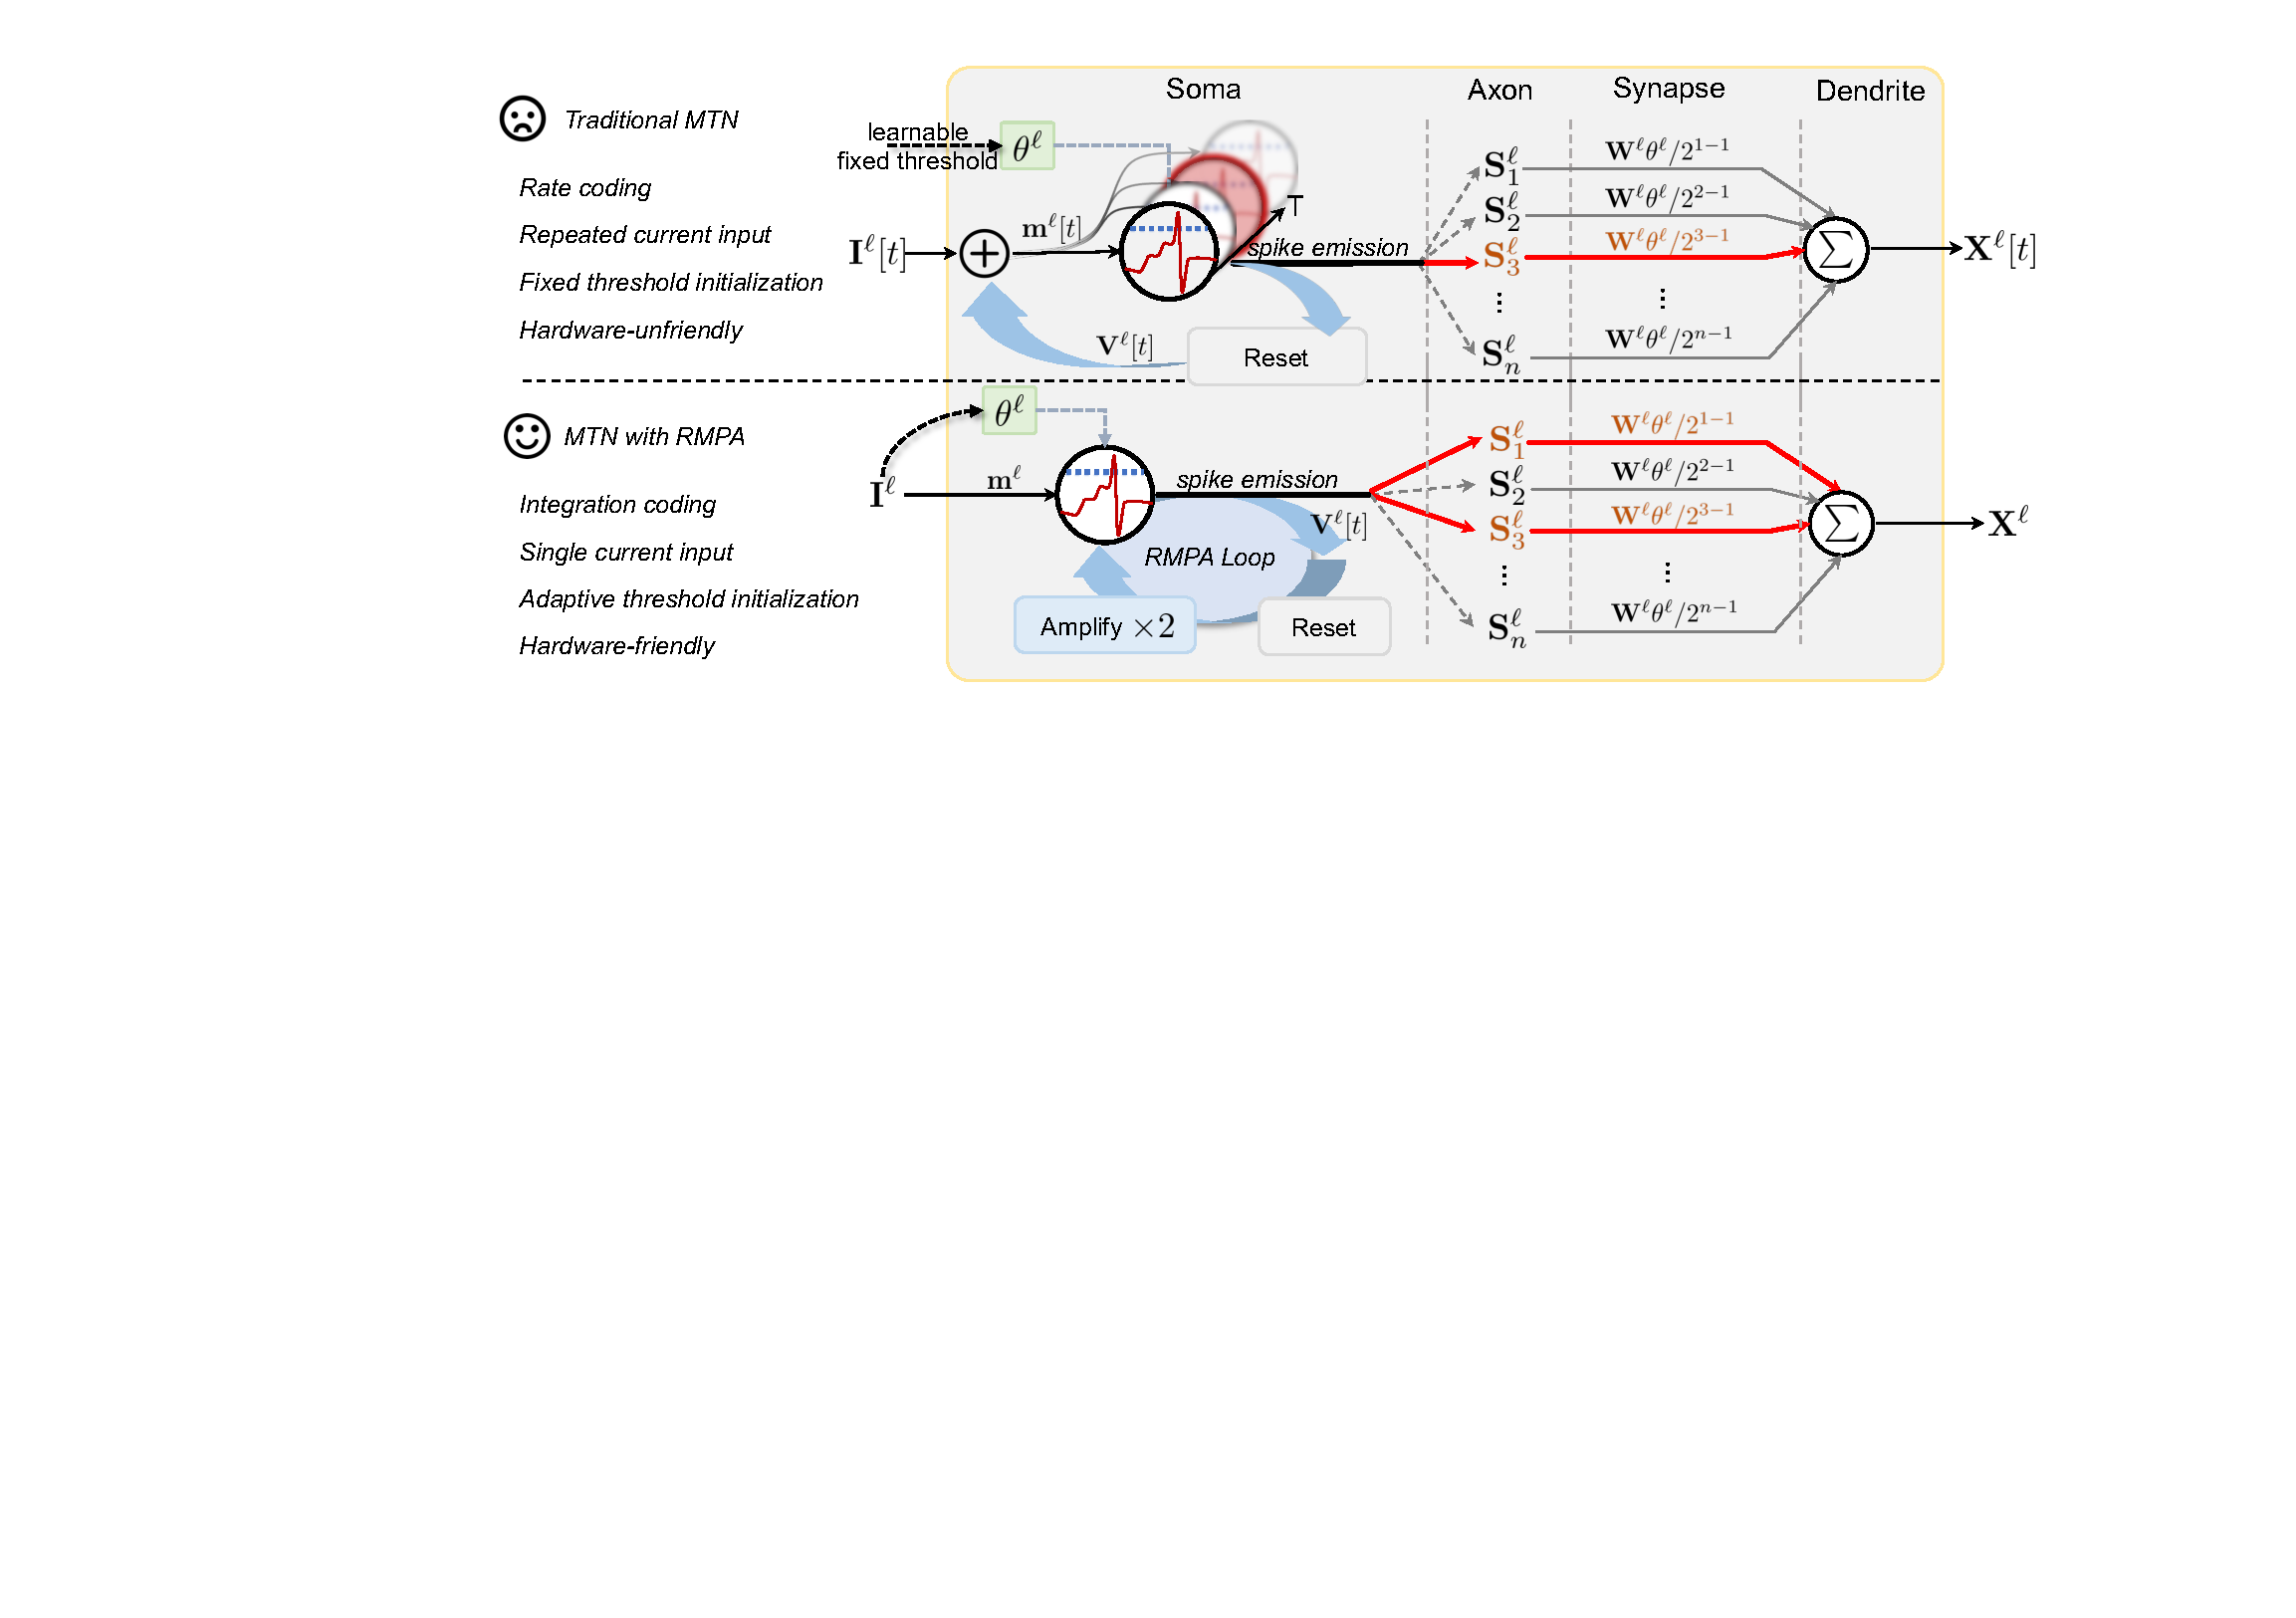
\includegraphics[width=1.0\linewidth]{Figs_new/01-neuron.pdf}
    \caption{Comparison between the traditional MTN and the proposed MTN with RMPA. \textbf{Upper}: For the traditional MTN, the input current is injected at each timestep, necessitating repeated accumulation operations of the input. 
    The neuron maintains $2n$ pre-set thresholds and compares its membrane potential against all of them to determine which spike to fire. 
    This results in redundant storage and computational overhead for threshold comparison per time step. 
    %The residual membrane potential is passively consumed over many timesteps, leading to information redundancy. 
    \textbf{Lower}: For the proposed MTN with RMPA, the input current is injected only once at the beginning, requiring no additional accumulation operation. 
    Instead of comparing against multiple thresholds, the neuron adaptively sets the only threshold $\theta^\ell = 2^p$ based on the input strength (Eq.~\ref{eqa:thres}). 
    At each timestep, a spike is fired if the residual potential after doubling exceeds $\theta^\ell$.
    Thus, only one threshold comparison is required, greatly reducing the computational overhead and the storage overhead from $\mathcal{O}(n)$ to $\mathcal{O}(1)$. %per timestep. %In this way, the residual potential of our MTN is actively amplified rather than passively consumed, making the error convergence speed of our MTN exponentially faster than that of the traditional MTN. (Proposition~\ref{prop:rmpa-mtn-error-bound}).
    }
    \label{Integral_Coding}
\end{figure}

% The dynamics of the integration coding-based MTN are illustrated in Fig.~\ref{Integral_Coding}. Unlike rate coding-based neurons, which receive input at every timestep, the integration coding-based MTN accepts input only once, so the input current $\mathbf{I}^l$ directly serves as the initial membrane potential $m^l = \mathbf{I}^l$.
The dynamics of the integration coding-based MTN are illustrated in Figure~\ref{Integral_Coding}. Conventional rate coding-based neurons accumulate input current at every timestep, whereas the integration coding-based MTN receives input only once, so the input current $\mathbf{I}^\ell$ directly initializes the membrane potential $m^\ell = \mathbf{I}^\ell$.
Afterwards, the neuron identifies the largest 
threshold that triggers spike emission, aligned with the binary structure of floating-point numbers 
(\hwrevised{the detailed description is in  Subsection} ~\ref{subsec:spike-gen-via-fp16-binary-parsing}). At the beginning, the base threshold $\theta^\ell$ is set and followed by a soft reset according to Eq.~\eqref{eqa:thres}:
\begin{equation}
\label{eqa:thres}
\theta^\ell = 2^p \text{ where } p = \max\{p \mid 2^p \leq \mathbf{m}^\ell,\ p \in \mathbb{Z}\}, \quad\mathbf{V}^\ell = \mathbf{m}^\ell - \frac{\mathbf{S}_i^\ell \theta^\ell}{2^{i-1}},
\end{equation}
% \begin{equation}
% \label{reset}
% \mathbf{V}^l = m^l - \frac{\mathbf{S}_i^l \theta^l}{2^{i-1}},
% \end{equation}
where $i$ indicates the loop index of RMPA.
In each subsequent iteration, $\mathbf{m}^\ell$ is set to the post-reset membrane potential $\mathbf{V}^\ell$.

% Under conventional rate coding, the neuron would repeat the integrate-fire-reset cycle at each timestep, passively waiting for the residual membrane potential to be incrementally consumed over many steps. The RMPA mechanism proposed in this work resolves this inefficiency. 
% As illustrated in Figure~\ref{Integral_Coding}, t
The RMPA-based MTN iteratively generates sub-threshold spikes from the residual membrane potential, progressively reducing the quantization error. Each spike generation requires only a bit-shift and a single comparison against the base threshold $\theta ^\ell$, eliminating storing a large number of thresholds. Formally, the firing rule is defined as Eq.~\eqref{eqa:spike}:
\begin{equation}
\label{eqa:spike}
\mathbf{S}_i^\ell = \mathrm{MTH}_{\theta,n}(\mathbf{m}^\ell, i) = 
\begin{cases}
1, & \text{if } \mathbf{m}^\ell \cdot 2^{i - 1} - {\theta ^\ell} \ge 0\, \\
0, & \text{otherwise}
\end{cases}.
\end{equation}

A soft reset is then applied as defined in Eq.~\eqref{eqa:thres}. Once the membrane potential reaches zero or the prescribed number of iterations is exhausted, the neuron decodes the emitted spike sequence to produce the total output signal of layer $\ell$:
\begin{equation}
{\mathbf{X}}^{\ell} = \sum_{i}\mathbf{S}_i^\ell \mathbf{W}^\ell \frac{ \theta^\ell}{2^{i-1}}.
\end{equation}
To further illustrate the dynamics of RMPA, a concrete example is provided in Appendix~\ref{sec:rmpa_example}.
%We illustrate the internal dynamics of RMPA with a concrete example.

% RMPA example moved to Appendix~\ref{sec:rmpa_example}.

%A concrete walkthrough of the RMPA dynamics with $x = 1.4$ is provided in Appendix~\ref{sec:rmpa_example}.

%We illustrate the internal dynamics of RMPA with a concrete example. Consider an input $x = 1.4$. According to Eq.~\eqref{eqa:thres}, the threshold $\theta^\ell$ is set to $1$ ($2^{p}$, $p=0$). After a spike of $\theta^\ell=1$ is emitted, it leaves $\mathbf{m}^\ell=1.4-1$ as $0.4$ and the index $i$ of RMPA loop as $1$. In the second iteration, $\mathbf{m}^\ell$ is doubled to $0.8$ and $i$ advances to $2$; since $\mathbf{m}^\ell = 0.8 < \theta^\ell=1$, no spike is emitted. In the third iteration, $\mathbf{m}^\ell$ is doubled to $1.6$ and $i$ advances to $3$; since $\mathbf{m}^\ell = 1.6 > \theta^\ell=1$, a spike of $\theta^\ell / 2^{i-1}= 0.25$ is fired and $\mathbf{m}^\ell$ is reset to $1.6 - 1 = 0.6$. At this point, the total encoded value is $1 + 0.25 = 1.25$, with residual membrane potential $\mathbf{m}^\ell = 0.6$. The remaining encoding error is $1.4 - 1.25$, the same as the result of $\mathbf{m}^\ell / 2^{i-1} = 0.6 / 4$, which decays exponentially with increasing iterations.

% Our method reduces threshold storage from $2n$ stored thresholds to $\mathcal{O}(1)$, with correspondingly fewer I/O operations. In contrast to rate coding, integration coding-based MTNs actively exploit the residual membrane potential to suppress quantization error, which underlies their accuracy advantage.
Our proposed neurons offer two key advantages: (i) threshold storage is reduced from $2n$ to $1$, with a corresponding reduction in I/O operations; (ii) unlike rate coding, integration coding-based MTNs actively exploit the residual membrane potential to suppress quantization error, which is the fundamental source of the accuracy gain.

\begin{proposition}[Error Bound of RMPA-based MTN]
\label{prop:rmpa-mtn-error-bound}
    The encoding error of rate coding is bounded by
    $\varepsilon_{\text{rate}} < \theta/2T,$
which decays linearly with $T$. In contrast, the proposed PRIME encoding attains a bound $\varepsilon_{\text{PRIME}} < \theta/2^{T \cdot D + 1}$, which decays exponentially with $T$, where $\theta$ denotes the spike threshold, $T$ \hwrevised{is} the number of inter-timesteps, and $D$  \hwrevised{is} the number of concurrent intra-timestep spikes.
\end{proposition}

% \begin{proposition}[Error Bound of the RMPA-based MTN]
% \label{prop:rmpa-mtn-error-bound}
%     The encoding error of conventional rate coding is bounded by
%     $\varepsilon_{\text{rate}} < \theta/2T,$
% which decreases only linearly with $T$. In contrast, the proposed PRIME encoding achieves an exponentially tighter bound of
% $\varepsilon_{\text{PRIME}} < \theta/2^{T \cdot D + 1},$
% where $\theta$ denotes the spike threshold, $T$ the number of inter-timesteps, and $D$ the number of concurrent intra-timestep spikes.
% \end{proposition}

% \paragraph{Proof Sketch.}
% In rate coding, after $T$ accumulation steps, $T \cdot \mathbf{I} = \theta \cdot N_{\text{spike}} + \mathbf{m}_{\text{rest}}$, giving error $\varepsilon = \mathbf{m}_{\text{rest}}/T < \theta/2T$ (with optimized initialization~\cite{hao2023bridging}). In integration coding, the input is applied once and the residual is amplified: after $n$ amplifications, $\mathbf{I} = \sum_i \theta/2^{n_i} + \mathbf{m}_{\text{rest}}/2^n$, yielding $\varepsilon < \theta/2^n$. Since $n \geq T \cdot D$, and the carry mechanism halves the error, we obtain $\varepsilon < \theta/2^{T \cdot D + 1}$. The full proof is in Appendix~\ref{sec:error}.


\hwrevised{The full proof is given in Appendix~\ref{sec:error}.} Accordingly, the error bound of our proposed MTN is significantly tighter than that of conventional MTN: for instance with $T=2$ and $D=3$, the error bound of PRIME is $\theta / 2^{7} = \theta / 128$, which is $32\times$ tighter than the rate coding bound of $\theta / 4$. 

\subsection{Hardware-efficient Inference}
\subsubsection{Spike Generation via Direct FP16 Binary Parsing}
\label{subsec:spike-gen-via-fp16-binary-parsing}
%%%强调公式10中得到的脉冲实际上可以通过读取fp16小数位实现,前面加一些描述初试阈值获取的部分，和这里对应
Here we describe how the spike generation process is  bound to the binary representation of FP16 data, eliminating conventional membrane potential computation. The key is that each field of the FP16 format: sign, exponent, and mantissa can be mapped to the threshold and the spike corresponding to Eq.~\eqref{eqa:thres} and ~\eqref{eqa:spike}, enabling a purely read-based spike emission mechanism.

A normalized FP16 floating-point number is represented as:
\begin{equation}
    x_{\textbf{10}} = (-1)^{S} \times 2^{E-15} \times \left(1 + \sum_{j=1}^{10} M_j \times 2^{-j}\right),
\end{equation}
where $S$ is the 1-bit sign, $E$ is the 5-bit exponent ($1 \leq E \leq 30$), and $M_1 M_2 \cdots M_{10}$ is the 10-bit mantissa with an implicit leading 1. 
% The discussion below focuses on normalized numbers; subnormal values ($E=0$), infinity, and NaN ($E=31$) are handled separately as special cases.
In the first cycle, the implicit leading 1 of the FP16 representation is directly emitted as the first spike, and the sign bit $S$ together with the exponent $E$ determines the corresponding threshold $\theta_1 = (-1)^{S} \times 2^{E-15}$. Starting from the second cycle, the position of the first 1 in the remaining mantissa is located using a leading-one detector (LOD), a well-established combinatorial logic module in digital circuit design. If the first 1 is found at position $k$ (counting from the most significant bit, $k = 1, 2, \ldots, 10$), the RMPA loop runs $k$ times and the corresponding threshold for the emitted spike is $\theta_k = (-1)^{S} \times 2^{E-15-k}.$ That is, position $k$ directly encodes the scaling factor $2^{-k}$ relative to the initial threshold, without any explicit computation. After the spike is emitted, the bit at position $k$ is cleared, and the LOD is applied to the updated mantissa in the next cycle to find the next 1. This process repeats until all cycles are exhausted or the mantissa becomes zero. Unlike the traditional ANN-to-SNN approaches that require the full subtract-compare-conditional updates, this method simplifies each cycle to LOD lookups followed by a bit-clear operation, significantly reducing computational cost.

% which require a full subtract, compare, and conditional update per cycle, each cycle here reduces to a single LOD lookup followed by a bit-clear operation, resulting in significantly lower hardware overhead.

\begin{figure}[ht]
    \centering
    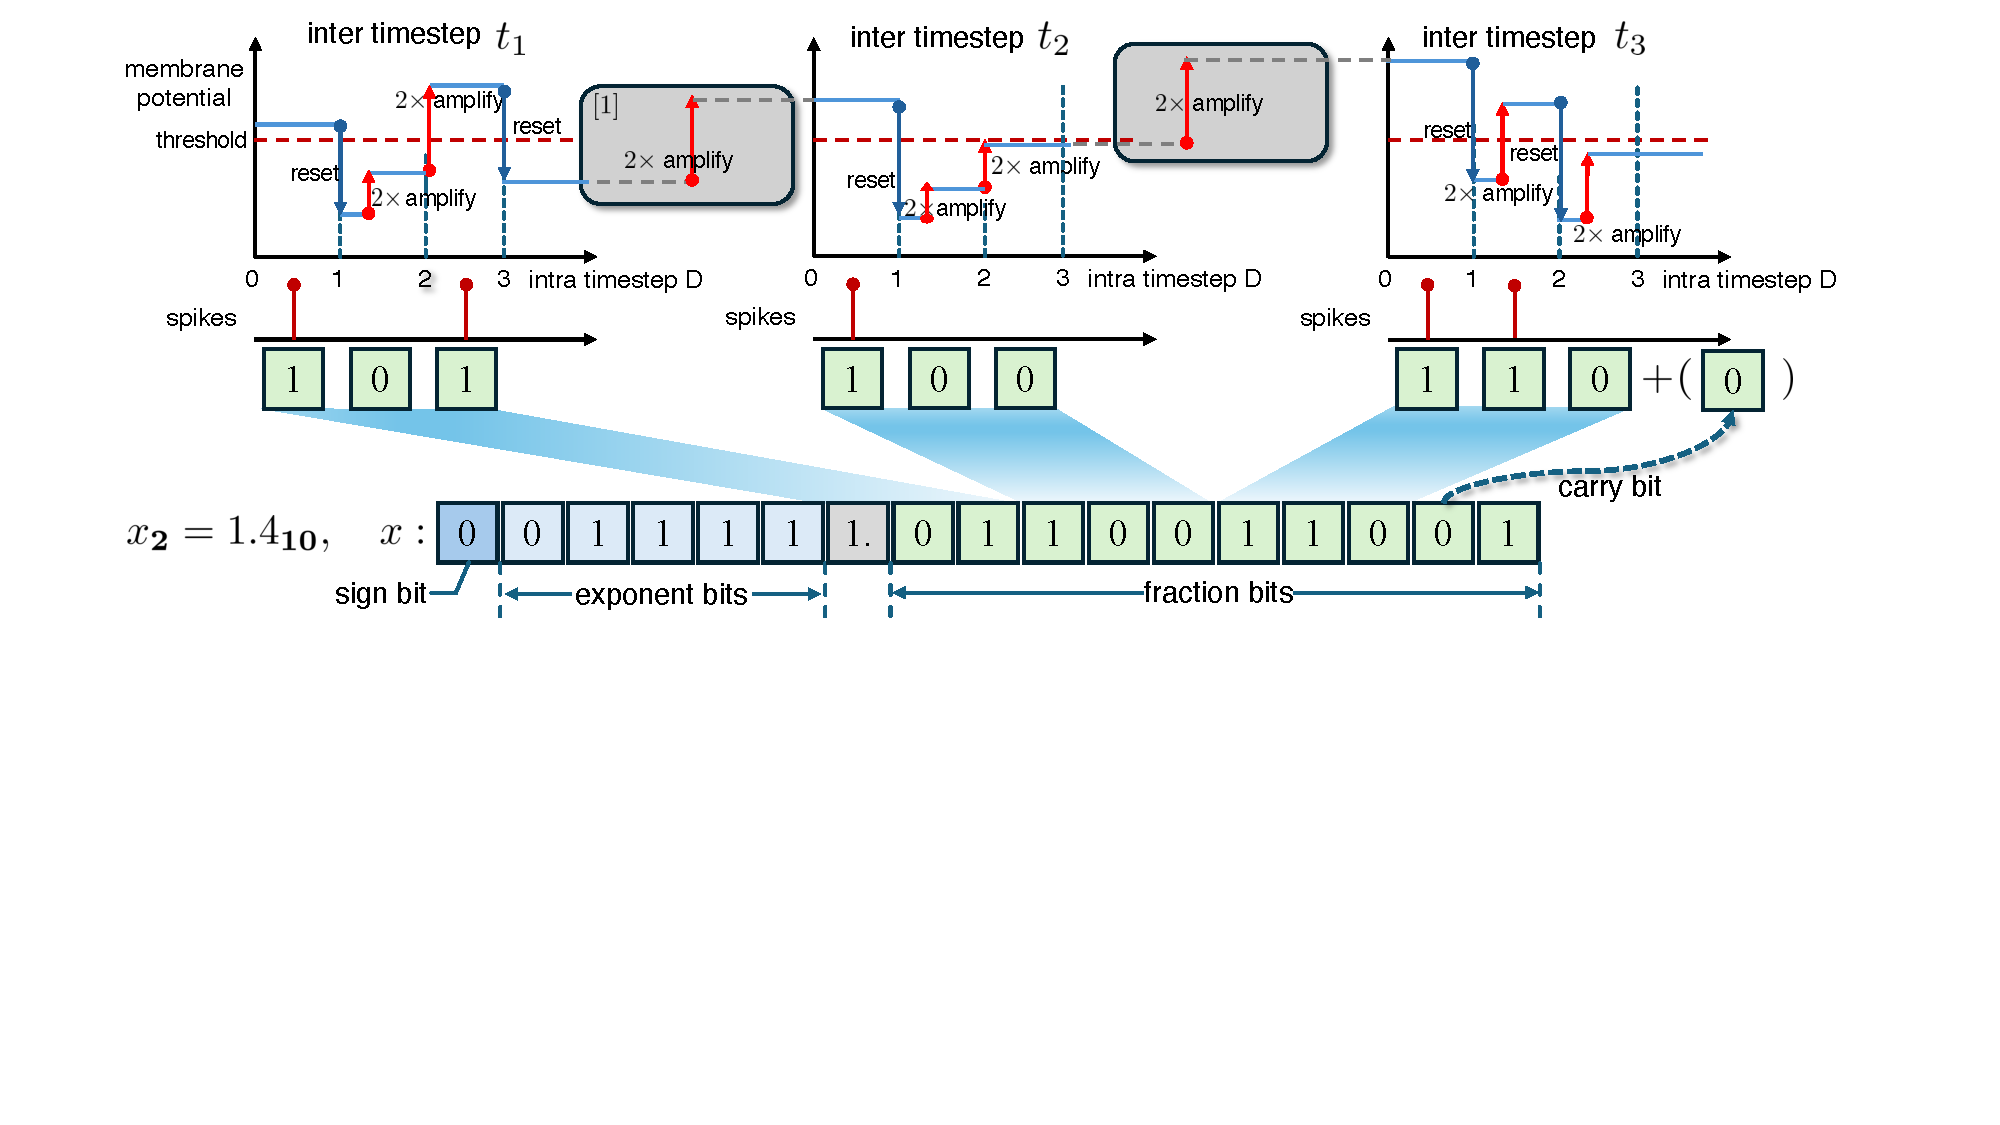
\includegraphics[width=1.0\linewidth]{Figs_new/figuers_1.pdf}
    %%%图例里面引用一下前面的放大过程，让软硬件部分结合的更好
    \caption{Parsing the FP16 representation of 1.4 into spikes with D=T=3. The first inter-timestep emits the implicit 1 concatenated with the leading 2 mantissa bits at threshold $\theta = (-1)^{S} \times 2^{E-15-(D-1)}$; the second uses the LOD to locate the first 1 in the remaining 8 bits, reads D bits from that position as the spike value, and shifts the threshold accordingly. $^{[1]}$ The number of amplifications is not strictly one. It equals the bit-offset of the next leading 1 from the end of the current $T$-bit group.}
    \label{fig:spikes2fp16}
\end{figure}

We present an example of parsing the FP16 data of 1.4 in Figure~\ref{fig:spikes2fp16}. We refer to $D$ as the intra-timestep spike dimension, which controls how many bits are emitted within a single timestep, and $T$ as the number of inter-timesteps, which controls how many successive timesteps are used to encode a given value. In the basic case ($D=1$), each timestep emits a 1-bit spike indicating whether the threshold is met. This paradigm further supports multi-bit spike emission by reading $D$ consecutive bits at a time, rather than a single bit. When $D > 1$, each spike is a $D$-bit unsigned integer ranging from 0 to $2^D - 1$, representing 0 to $2^D - 1$ times the corresponding threshold. For example, when $D=2$, 2 bits are read per timestep, encoding spike values in $\{0, 1, 2, 3\}$; when $D=3$, 3 bits are read, encoding values in $\{0, 1, \ldots, 7\}$. In the last timestep, an additional bit (i.e., the (D+1)-th bit) is read beyond the D-bit spike. This extra bit is then added to the D-bit spike value, treated as an unsigned integer, to perform a carry operation, which is equivalent to a round-half-up operation, and further improves encoding accuracy without introducing a separate rounding stage.

At the hardware level, this intra-timestep expansion only requires widening the read window from 1 bit to $D$ bits; the LOD-based position finding and threshold determination remain unchanged. This multi-bit emission significantly increases the information density per timestep and is difficult to achieve in traditional ANN-to-SNN conversion algorithms, where each timestep is inherently limited to a binary fire-or-not decision.

% From a neuromorphic hardware perspective, the $D > 1$ mechanism maps directly to a \emph{graded-spike} encoding scheme that is compatible with both digital and mixed-signal neuromorphic architectures. In conventional neuromorphic designs, each neuron emits a binary spike (0 or 1) per timestep, and multi-bit information must be encoded across multiple timesteps, incurring latency overhead. In contrast, PRIME emits a $D$-bit unsigned integer spike per timestep, where the spike amplitude $s_t \in \{0, 1, \ldots, 2^D - 1\}$ directly represents a multi-level synaptic event. At the circuit level, this requires: (1) a $D$-wide read port on the mantissa register, which is a trivial extension of the single-bit latch; (2) a conditional shift-add module (CSAM) comprising $D$ multiplexers and a $(D-1)$-stage adder tree to compute $s_t \times F_w$; and (3) a trace-aligned accumulator that right-shifts and sums the partial products across timesteps. The CSAM replaces the $11 \times 11$-bit combinational multiplier array with $D$ simple MUX-adder pairs, reducing hardware area by $\sim 5\times$ for $D=3$. Furthermore, since each spike value $s_t$ is an unsigned integer, the synaptic multiplication $s_t \times w$ degenerates to at most $D$ conditional additions (one per set bit in $s_t$), which can be dispatched to a standard MAC array without modification. For the special case $s_t = 2^D - 1$ (all bits set), a single subtraction suffices (Appendix~\ref{sec:111}), ensuring that the worst-case latency per cycle is bounded by one addition.

A key advantage of this binary-parsing approach is that when $T \leq 2$, the two timesteps are data-independent: the first reads the implicit 1 and leading mantissa bits, while the second operates on the remaining bits through a LOD. Since the second timestep depends only on a predetermined bit range, both can be executed in parallel, effectively halving the latency.

\subsubsection{Efficient Multiplication Under Spike Traces}
%%%强调一下功耗比较节约，相比于常规的fp16加法
The spike generation mechanism described above decomposes an FP16 value into a sequence of weighted spikes over $T$ inter-timesteps. We now show how this decomposition naturally induces a hardware-efficient multiplication scheme: instead of performing a full $11 \times 11$-bit mantissa multiplication, the product $x \times w$ is computed incrementally through spike-driven conditional shift-add operations across timesteps.

\paragraph{Sign and Exponent.}
Given two FP16 operands $x$ and $w$, the sign and exponent of the product are computed in the standard manner. The output sign is obtained via a single XOR gate: $S_o = S_x \oplus S_w$, 
and the output exponent is $E_o = E_x + E_w - \text{bias}$, 
where $\text{bias} = 01111_2 = 15_{10}$. This requires only a 5-bit adder and a 6-bit subtractor, identical to a conventional FP16 multiplier. The key innovation lies entirely in how the mantissa product is computed, as described below.

\begin{figure}[ht]
    \centering
    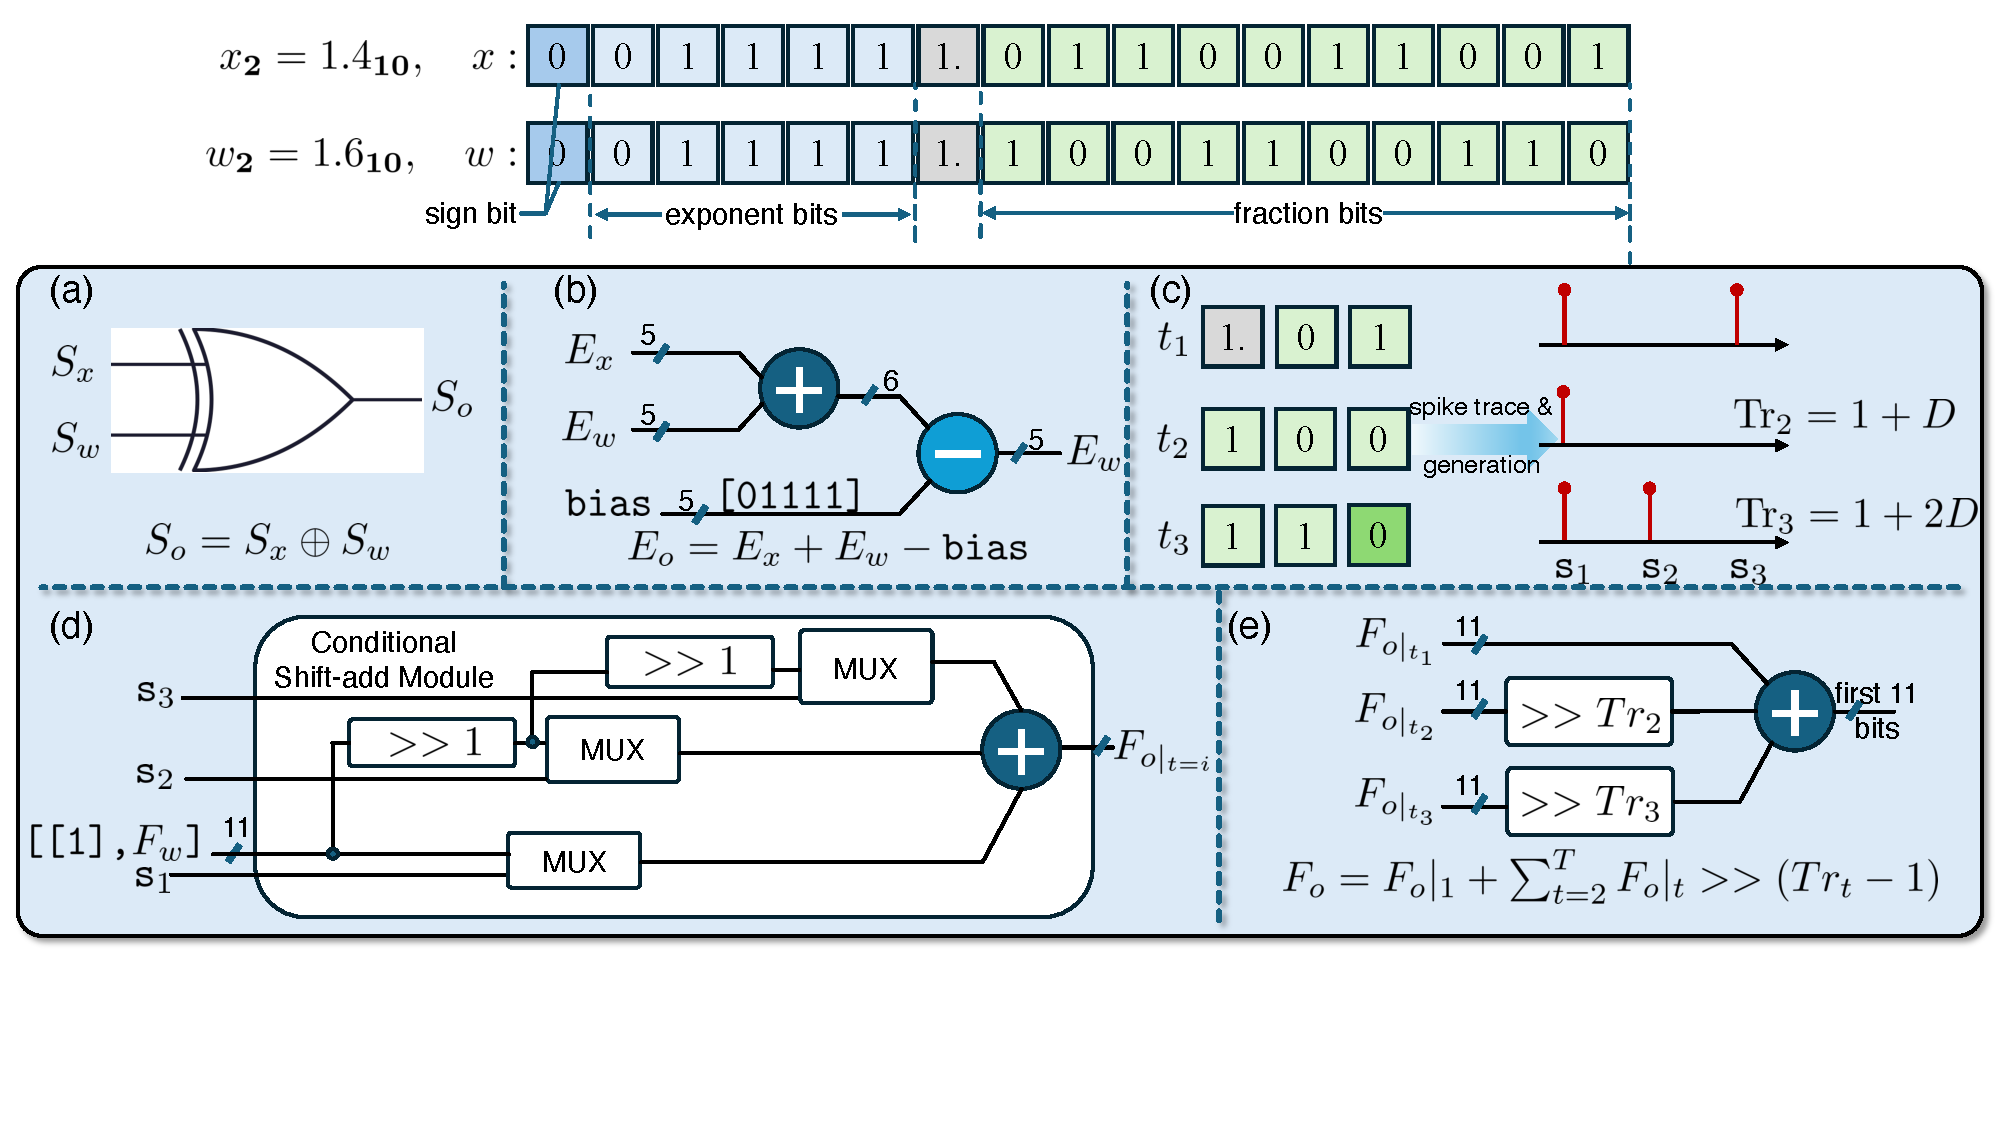
\includegraphics[width=1.0\linewidth]{Figs_new/figuers_2.pdf}
    \caption{Spike-driven FP16 multiplication. Sign, exponent, and mantissa of $x$ and $w$ are processed in parallel: \textbf{(a)} $S_o = S_x \oplus S_w$ via XOR; \textbf{(b)} $E_o = E_x + E_w - \text{bias}$ via a 5-bit adder and 6-bit subtractor; \textbf{(c)} the mantissa $F_x$ is decomposed into $T$ spikes $\{s_t\}$ with traces $\mathrm{Tr}_t = 1+(t-1)D$; \textbf{(d)} each partial product $F_{o}|_t = s_t \times F_w$ is computed by a Conditional Shift-add Module of MUXes and an adder tree, replacing the $11\times11$ multiplier array; \textbf{(e)} partial products are trace-aligned via right shifts and summed to form $F_o$, truncated to 11 bits.}
    \label{fig:calc}
\end{figure}

\paragraph{Mantissa Decomposition via Spike Traces.}
Let $F_x = 1.M_{x,1} M_{x,2} \cdots M_{x,10}$ denote the full mantissa of $x$ (including the implicit leading 1), and similarly $F_w$ for $w$. The spike generation process of the previous subsection decomposes $F_x$ into $T$ spike values $\{s_t\}_{t=1}^{T}$, each being a $D$-bit unsigned integer, with an associated trace value $\mathrm{Tr}_t$ that records the bit-position offset of the $t$-th spike relative to the binary point. Specifically, the first spike $s_1$ is composed of the implicit 1 together with the first $D-1$ mantissa bits, and the corresponding trace is $\mathrm{Tr}_1 = 1$. For subsequent timesteps $t \geq 2$, the LOD identifies the starting position of the next group, and $D$ consecutive bits are read as $s_t$. The trace value satisfies:
$
\mathrm{Tr}_t = 1 + (t-1) \times D,
$
when the mantissa bits are densely packed (i.e., no intervening zeros between groups). Under this decomposition, the mantissa can be reconstructed as $F_x = \sum_{t=1}^{T} s_t \times 2^{-(\mathrm{Tr}_t - 1)}.$ 
Substituting into the mantissa product yields:
\begin{equation}\label{eq:mantissa_product}
F_o = F_x \times F_w = \sum_{t=1}^{T} \underbrace{(s_t \times F_w)}_{\triangleq\; F_{o}|_t} \times 2^{-(\mathrm{Tr}_t - 1)}.
\end{equation}
This factorization reveals that the $11 \times 11$-bit mantissa multiplication is decomposed into $T$ smaller multiplications of a $D$-bit spike $s_t$ by the 11-bit mantissa $F_w$, followed by trace-aligned accumulation. Each per-timestep partial product $F_{o}|_t = s_t \times F_w$ is a $D$-bit $\times$ 11-bit multiplication, which can be efficiently realized by a Conditional Shift-add Module as illustrated in Figure~\ref{fig:spikes2fp16}(d). Let $s_t = \sum_{j=1}^{D} b_j \times 2^{D-j}$, where $b_j \in \{0,1\}$ are the individual bits of the $D$-bit spike. Then:
\begin{equation}\label{eq:shift_add}
F_{o}|_t = s_t \times F_w = \sum_{j=1}^{D} b_j \times (F_w \gg (j-1)),
\end{equation}
where $\gg$ denotes logical right shift. Each term $b_j \times (F_w \gg (j-1))$ is implemented by a multiplexer (MUX) controlled by $b_j$: when $b_j = 1$, the shifted value $F_w \gg (j-1)$ is selected; when $b_j = 0$, zero is selected. The $D$ selected values are then summed by an adder tree. This conditional shift-add structure replaces the combinatorial multiplier array with $D$ MUXes and a $(D-1)$-stage adder tree, significantly reducing the hardware area. Note that when $\text{spike} = 111$, the multiplication can be computed more efficiently by rewriting it as $1000 - 0001$, requiring only a single subtraction. A detailed derivation is provided in Appendix~\ref{sec:111}.
 
\paragraph{Trace-aligned Temporal Accumulation.}
As shown in Figure~\ref{fig:calc}(e), the final mantissa is the trace-aligned sum of the $T$ partial products $F_{o}|_t$: 
\begin{equation}\label{eq:temporal_accum}
F_o = F_{o}|_1 + \sum_{t=2}^{T} F_{o}|_t \gg (\mathrm{Tr}_t - 1).
\end{equation}
The right shift $\gg (\mathrm{Tr}_t - 1)$ aligns the $t$-th partial product to the correct bit position relative to the first partial product, and the final sum is truncated to the first 11 bits to produce the output mantissa. This temporal accumulation directly mirrors the dynamics of synaptic integration in SNNs: each incoming spike $s_t$ triggers a weighted response $F_{o}|_t$, and the trace $\mathrm{Tr}_t$ governs the temporal decay (realized here as a right shift) before the responses are accumulated at the output neuron. 

The Spike Generation via Direct FP Binary Parsing, together with the Spike-driven Multiplication, yields significant energy and data-transmission savings. The detailed energy analysis is given in Appendix~\ref{sec:energy}.

%As shown in Appendix~\ref{sec:energy}, under the setting $T = 2$, $D = 3$, the Spike Generation via Direct FP16 Binary Parsing and the Spike-driven Multiplication yield significant energy and data-transmission savings. We report results relative to both FP32 and FP16 baselines. FP32 multiplication consumes 3.7\,pJ per operation~\cite{energy} and is widely adopted as the energy reference in neuromorphic computing literature~\cite{energy, energy_scale}; FP16 multiplication consumes 1.1\,pJ and represents the most common reduced-precision baseline in modern accelerators. At $T{=}2$, $D{=}3$, the per-operation energy is 0.390\,pJ,  corresponds to \textbf{10.5\% of FP32} and \textbf{35.5\% of FP16}; the inter-layer bit-transmission cost is 13 bits,  \textbf{40.6\% of FP32} and \textbf{81.3\% of FP16}. Detailed energy breakdowns for both FP32 and FP16 baselines are provided in Appendix~\ref{sec:energy} (Table~\ref{tab:power_consumption}).

%Moreover, PRIME framework is not limited to FP16 operands; it also supports other formats such as INT4 and FP8. The same binary-parsing and spike-driven multiplication principles apply to these formats, and energy and bit-transmission analyses are provided in Appendix~\ref{sec:fp8_int4} (Tables~\ref{tab:fp8_prime}, \ref{tab:int4_prime}, \ref{tab:flatquant_prime_llama2}).